\chapter{Introduction}

%- Intro biology
%- beskrivelse af opgaven
%- beskrivelse af batbox
%- beskriv streaming idea
as everything is considered as stream, it becomes naturally to also do online processing on th esound stream, and take the output as video streams(waterfall spectrogram)
%- Analyse
\todo{Set the scene - publishers/subscribers, define host, nodes etc.}
\section{Users}

\begin{itemize}
	\item Biologists
	\item Developers(users, Thor)
	\item Developers(Code, John)
	\item Supervisors
	\item Backend developers
\end{itemize}

\section{Use Cases}
\myparagraph{Porpoise}
Underwater recordings are used to record Porpoise to investigate how windmills affects the Porpoise live.
\begin{itemize}
	\item {\textbf{Long recordings:}}  Hydrophones are mounted on pillars to record where the mereswines swim. The initial hypothesis was, that windmills would inhibit whales from living in that area close to windmills. However it turned out, that the whales started to breed near the windmills. Recordings are done for long periods of time.
	
	\item {\textbf{Short recordings}} During experiments, recordings of 1 min are done every 10 minute.

\end{itemize}

\myparagraph{Bats}

\todo{Insert image of batcage}
\begin{itemize}
	\item \textbf{Long recordings:} Long time recordings are used when investigating the behavior of bats in their natural habitat from ground. An example of this is when the new hospital is build in Odense. By putting up microphones the bats’ behavior can be recorded and compared to the behavior after the hospital has been build.
	
	 \item \textbf{Short recordings} Short recordings are used in Panama, as the recording boxes are not easy accessible to get near as they are mounted deep in forests. Due to lack of accessibility of the recordingsystem, the hard drives of the recordingboxes cannot easily be accessed when needed to be replaced. Therefore, they instead want to do a recording of 10 min each hour.

	\item \textbf{Trigger recordings} Trigger recordings ares used doing experiments with bats. The biologists have a bat cage, where they can conduct different experiments with bats. Sometimes it takes long before the bat does what is intended to do, so instead of doing long recordings, the biologist uses trigger recordings. When the biologist observes the bat do as intended, the biologis pushes a button, and the system saves x seconds before and after he triggered the recording. This way, he ensures that his recording contains the interesting bit, and he does not have to go through a huge amount of data, to find what he is looking for.
\end{itemize}
\todo{Figure of trigger recording}

\myparagraph{Frogs}
\begin{itemize}
	\item \textbf{Long recordings:} Frogs are recorded in their natural habitat in order to verify theoretical models of their croaking. The recordings are usually done overnight where the croaking is saved to a local disk. The bat boxes record frogs by using 8 microphones mounted in different heights and different distances. This data collected from the batboxes can be used to verify models in RANA.
\end{itemize}


\myparagraph{Skype for birds}
\todo{Insert image of setup}
\begin{itemize}
	\item \textbf{Long recordings} The idea is to tamper with communication between two Zebra Finches to understand how the tutor bird teaches the younger bird how to chirp. The batboxes are used to record the sound from one birdcage which is then played in the second birdcage. Between recording and playing, the sound can be manipulated by an AI. Recordings are played in realtime and stored for later processing. The project also concerns with tampering with two video streams(one in each direction) between the two bird cages. 
\end{itemize}
% kasser, 


\myparagraph{Drones}
The recording system is mounted on drones in order to:
\begin{itemize}
	\item \textbf{Trigger recording}Emulate the localization of a bat by emitting ultrasonic sounds. A trigger recording is started when the ultrasonic sound is emitted, such that the bounce of the emitted signal can be recording. The bounces from the signal will arrive at the batbox again within 30 ms.
	
	\item \textbf{Long recording} Point  the drone in the direction of a bat. Using multilateration, the position of the bats is estimated. GNSS will be used to synchronize the time of the batboxes. 
\end{itemize}

\myparagraph{View recordings live}
During setup of a new system, is it desired to to view the recorded data in "realtime". This would ease the setup as the microphones' position can be adjusted while watching the live processing of the data, and it would verify the system is working
Furthermore it is wanted to be able to demonstrate the system to students or other people who has interest in the functionality of the system.

\myparagraph{Calibration}
In many setups, calibration is required to know the properties of the microphones or the relative location of the microphones.
\begin{itemize}
	\item \textbf{Geometric Calibration} When the system is used to obtain the position of one or many sound sources, the microphones need to be calibration with respect to each other. By generating several sounds which are recorded by each microphone used in the setup, the position of each microphone can be estimated using multilateration. This is often needed with multiple recording boxes.
	
	\item \textbf{Frequency Calibration} Since the microphones are not linear at all frequencies, the microphones can be calibrated such that a filter can be applied to compensate for the nonlinearity.
This is done by having a speaking pointed towards a microphone, where the speakers emits sounds at known frequencies. These sounds are recorded and used to create an equalizer that can be used to compensate

\end{itemize}

\myparagraph{Data syntheses}
Either during capture or after the capturing, processing of the must be done in order to extract knowledge from the recordings.

\begin{itemize}
	\item \textbf{Data push} In some applications, the batboxes will have access to a backend’s network where data can be streamed as they are recorded. In other applications the data is saved to a local disk, which is then manually connected to the backend where data needs to be transferred to the backend.
	
	\item \textbf{Data Analysis} It should be possible to stream data to Abacus, where it can be analyzed and processed, but should also be possible to post process the data.

	\item \textbf{Data publish} When data is processed, whether it is in realtime or post-analysis, it should be presented and published in a nice way such that biologists can easily get an overview and see important features from the recorded data. Data can be exported in different formats which could for instance be to a website such that bats position can be viewed on an online map.

\end{itemize}


\myparagraph{Other sensors}
Other types of sensors should be added to the system as metadata. In some applications a GPS should be used to synchronize time, but also to know the position of the batboxes. Several parameters such as temperature, humidity etc. affects the sound measurements, so those parameters should be saved with the recordings as metadata. 

\section{Existing system}

\begin{figure}[h!]
	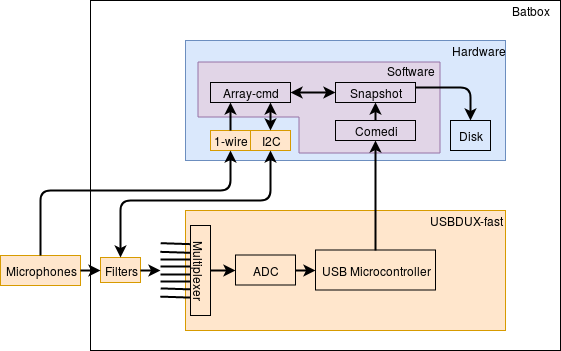
\includegraphics[width=1\textwidth]{figures/existing-system-overview.png} 
\end{figure}

\todo{Google howto export figure from draw.io to latex}

\subsection{Current setup}

As shown in section <Use-cases>, the existing system comprises of the following nodes:

snapchot is responsible for getting the auto from the usbdux/comedi module and writing the samples into files. When snapshot is initialized, it will record samples, however data is only saved to a circular buffer until it is told to write the buffer into a file. The snapshot will save part of the circular buffer to a file when it receives a “snap” command. This gives the ability to get a recording, consisting of data from a predefined time before it receives the “snap” command. Snapshot is designed to not miss out samples from the ADC.

grab has overlapping responsibility with snapshot, however: grab outputs samples to stdout and not by writing to any files. Furthermore, the implementation of the grab node is much more simple, as it has no need to maintain a circular buffering and thereby implement less memory management. If the consuming process blocks its stdin, grab will loose samples.

snapchat is responsible for communicating with snapchot and/or array-cmd depending on the application. Snapshot is run from CLI where it takes its input as parameters, and outputs by connecting to the snapshot/array-cmd.

cmd-arrays responsibilities are listed below:
Setting up the usbdux 
Handles GPIO to HMI
Saving meta-data for recordings
Determine mode of operation
Handling uuid generation
Handling recording paths
Handling connected microphones.
Being the interface to the system.
UDP + ZMQ
Hardware communication with:
LTC2637(DAC) over I2C
See flowchart of array-cmd.

trig instructs the snapshot when to do a snapshot by constructing and sending a “snap” command to either cmd-array or snapchat.

array is a script that hides the complexity of the system to ease the interface for the biologists. It is capable of initializing the system, listing connected microphones, setting options on the microphones, starting/stopping recordings etc.

Hardware - trigger line(master/slave setups)
Communication between nodes.
The interface to the recording system is either UDP or ZMQ using request/reply-pattern. Communication between the demons and CLI tools is ZMQ. Communication between threads in snapshot is also using ZMQ, however using push-patterns as ZMQ is used to do logging from busy threads.

Startup and supervision
All demons are run under supervision from the debian runit package. The runit package is both responsible for starting the nodes during startup, but also to keep the nodes running in case one of them crashes. Since runit does not provide any control of the order of startup, some fiddling has been made in order to start the snapshot and array-cmd in the proper order. From array-cmd’s run file, it tells snapshot’s supervisor, to start running.

Table of running/non-running processes.


Node name
Impl.Language
Running one-shot
Running forever
Running when used(long term)
snapshot




X


snapchat


X




grab






X
trig


X
X
X
array-cmd




X




Requirements:
Add other types of sensors (GPS, humidity, temp etc.)
Send recordings to backend when PI is online
The PI should not require internet to do recordings
Support for different hardware versions of the batbox.
Software should run on RPI
Snapshot should also be able to run on Intel in cases where powerfull enough RPI is not available.




Move files to more sensible structure
Describe different hardware versions as this makes up requirement for probing hardware

\todo{Describe and make diagrams of how to userlands tools talk through comedi modules to hardware}
\subsection{Hardware versions}
Version 1
Version 2A
Version 2B
Drone
\todo{Describe hardware. Make diagrams of the connected components}


%\myparagraph{Interface}
%As biologists are the typical user of the system, a userfriendly webinterface should be provided. Designing and implementing this is out of the scope of the report. However, it is kept in mind

\newpage
\chapter{Analysis}
\section{Design requirements}
The proposed system is designed with the concepts of the unix philosophy in mind
\begin{itemize}
	\item Programs should do one thing, and do it well
	\item Programs should be able to work together
	\item Programs should be capable of taking streams of text as input
\end{itemize}

By complying with the three ideas from above, the system should consist of multiple small programs that can be put together in different ways to serve different purposes.

Since the system is developed for biologists, it should be easy to use and require minimum intervention to get it running. Ideally the system should be “plug and play” such that biologists can take the number of recording boxes required for their application and put it all together without the need to configure software on any of the boxes. \todo{Add Extensibility somewhere, maybe not due to maintainability}



\todo{Add: Write as little code as possible, use already existing code maintained by other developers}
\todo{add: Should be a requirement that it should be easy to write new nodes. Should not require an interface to send commands, should be self-contained as possible.}

Furthermore the system should also be:

\begin{itemize}
	\item Maintainability
As other people will improve the system in the future, it should also be easy to maintain. This will almost happen automatically if the “unix design rules” are kept in mind during design and development.
\item Modular
The system should consist of multiple small programs so that it can be used in all existing use-cases but also those that might come in the future.
\item Reusability
As much code should be as reusable as possible in order to avoid implementing the same functionality multiple times.
\item Extensible
    By implementing small programs, the system should be easy to extend in the future.
    If functionality is missing in one of the programs, it should be possible to create a new 
    program with the new functionality.
\end{itemize}

However splitting functionality into multiple modules will also be done with caution as it might come with the price of performance. Each time programs are split up, there is usually required some communication between the programs or some exchange of memory. The communication might turn out to be unnecessary performance consumption. Therefore splitting programs up is seen as simplicity(as it eases development and use) vs. performance.

% \section{Recording}
% stream data out
% timestamp for accurately compare streams\todo{verify with John}


\begin{figure}[h!]
	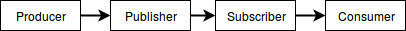
\includegraphics[width=1\textwidth]{figures/analysis-terminilogy-overview.png}
	\caption{Overview of nodes, to ease understanding of the terminology used throughout the following sections. It should be noted, that the producer and consumer is just programs producing and consuming streams without being aware of the protocols between the producer and subscriber.}
\end{figure}

\section{Streams}
% A streams is an abstraction, that hides the details in the communication between subscribers and publishers.
A stream is defined as coherent data, which is in the process of being transmitted. A stream does not conceptually have an explicit beginning or end nor does it necessarily have a header explaining the content of the stream. A stream can either be continuous or discrete which depends on the content of the stream. 


Given use case \ref{usecase:x}, the stream must be capable of comprising sound, text and video formats only relying on codecs available. As all streams are transmitted over multicast groups, the streams must be packet-oriented since they are transported as UDP packets.
As UDP packets might arrive out of order, or not arrive at all, the stream must be robust to lost packets, without loosing global knowledge of the stream.
TCP is not considered an option, as this would not take advantage of the multicast groups. TCP is connection-oriented meaning it would require a connection from each producer to each consumer, this would limit the number of consumers per producer due to the RPI's bandwidth limitation.

Both publisher and subscriber is stateless with respect to the data streams. However, they might both maintain a state about the metadata streams.

Since the stream is just data, there must be metadata available that describes the content of the streams. The streams must be described unambiguously, such that each stream can be differentiated from the other streams. Since the streams are to be recorded and replayed, metadata must also be available when the streams are replayed, in order to identify the streams when replayed. Therefore, the streams must be complete and depend on no external knowledge.
As the system will usually comprise of multiple streams, each stream must have a unique, sensible name used to refer to the stream. Furthermore it must have an unique identifier that allow streams to refer to eachother.
As in use case \ref{usecase:energizer}, where a node consumes a stream and produces a new stream, the new stream must explicitly specify its parent stream using the parent's unique identifier. This gives rise to model the streams as a forest of graphs, where each graph should always be an directed acyclic graph, in order to avoid streams that depend on themselves.

\todo{Figure of example graph}

\subsection{Producers and Consumers}
As streams may contain different formats, the producer and consumer must be agnostic to the content of the stream, and must handle the data to and from the stream.
Multiple consumers and producers must be able to subscribe and publish to the same multicast group, however the producer and consumer must give a warning, if the topic is already used by another producer. In order for this to work, the consumers and producers must implement a presence protocol, that detects the presents of other producers and consumers on a specific stream. This must be implemented in a way such that possible conflicts can be detected within X seconds from a producer/consumer is run, where X is specified as a parameter to the nodes.

As there is no designated master in the system, the producers must be designed such that that independently can find available multicast groups, without relying on too many well-known multicast groups. When a consumer is used to subscribe to a stream using the stream's unique name, the consumer must single-handedly be able to find the requested multicast group.
As producers and consumers unlikely joins multicast groups at the same time, the producer and consumers most be able to cope with nodes asynchronously joining and leaving multicast groups.

Both producer and consumer must be implemented as C-libraries and support bindings to other languages, to ease implementing new consumers and producers for future applications.

From use case \ref{sec:usecase:energizer}, the energy calculation should happen from bulk of samples corresponding to 1 ms. To ease the implementation of the energizer-node and future nodes, it should be possible to set the payload size of the publisher node. If the payload length of the stream corresponds to 1 ms of samples, the energizer node do not have to implement a buffer mechanism. If the length of the packet exceeds the practical limits of the network, the producer must give a warning. From the incoming data to the producer, and the outgoing data from the consumer, there should be no limit of the packet sizes.

As metadata is required, it must be possible to provide metadata to the publishers such that it can stream it to the subscribers. 

\subsubsection{Metadata}
% Analysis of metadata
	% Metadata 
	% Sequence number in packet.
	
	
Metdata can be split into three categories:
\begin{itemize}
	\item "PTR-record" is the metdata that concerns with pointing to a high bandwidth stream from the metadata stream.
	\item \textbf{Internal stream}-metadata describes the stream such as codec, sample frequency etc.
	\item \textbf{External strea}-metadata describes properties of the stream that relates to the source-node. In case of batbox this will be unique-id, microphone parameters
\end{itemize}
Metadata is required in order for the subscriber nodes to know the multicast address of high bandwidth streams. Metadata is also required to 

Metadata is required to describe the streams, the publisher and subscriber must be capable of sending and receiving metadata. The metadata should be considered a discrete stream as metadata is periodically transmitted as one-shot packets. As with the datastream, metadata will be sent as UDP packets, but to a well-known topic.
When metadata is published, it should have a checksum attached that allows detecting if the content of the metadata has changed during transfer.
 
Both the publisher and subscriber must be agnostic with respect to the semantics of the metadata meaning different formats such as JSON, XML etc. must be allowed to format metadata. The metadata should be provided during start of the publisher and repeated at a given rate specified as a parameter.  allowed to change


% Layers of metadata:
% - datastream contains metadata(seq id, 32 bit timestamp)
% - metdata on metadatastream(streamid, streamname, multicast stream)
% - Metadata regarding e.g batbox

\subsection{Requirements}
From the analysis, the following requirements can be extracted.
\subsubsection{Streams}
\begin{enumerate}
	\item The stream can be either continuous or discrete.
	\item The stream must comprise different datatypes only by relying on available codecs.
	\item The stream must be packet-oriented and stateless
	\item The stream must be transported over UDP
	\item The stream must be robust to UDP packets that arrive out of order or never arrive.
	\item The stream must be represented unambiguously
	\item Metadata must be provided by the publishers and be available to the subscribers 
\end{enumerate}

\subsubsection{Producer \& Consumer}
\begin{enumerate}
	\item The producer and consumer must be agnostic to the stream's payload.
	\item Multiple producers must send to the same multicast group.
	\item Multiple consumers must receive from the same multicast group.
	\item The producers and consumers must implement a presence mechanism to know about other producers and consumers.
	\begin{enumerate}
		\item It must takes a finite maximum number of seconds for a producer or subscriber to know who is present. The max time must be a parameter of each node.
		\item It must take a finite maximum number of seconds for a producer or consumer to detect whether a multicast group is in use, and if yes, by whom.
		\item It must assume nodes leaving a multicast group sends a "bye".
		\item It must be robust to "bye"-messages not arriving to all nodes.
		\item It must handle nodes joining and leaving at any arbitrary time.
	\end{enumerate}
	\item The producers must be able to find unused multicast groups single-handedly.
	\item Given a unique name of a stream, the consumer must be able to resolve the multicast address of the stream.
	\item Both producers and consumers must be able to cope with nodes joining asynchronously.
	\item The producer and consumer must be implemented in C and support language bindings.
	\item The payload length of the stream should be adjustable as a parameter on the producer nodes.
		\begin{enumerate}
			\item If the requested payload size is exceeded practical limits, a warning must be given.
		\end{enumerate}
	\item There should not be a limit of the packet size of the incoming data to the producer, or outgoing data from the consumer.
	\item The producer must support streaming provided metadata to the consumers.
	\item Both producer and consumer must be agnostic with respect to the semantics of the metadata.
\end{enumerate}

\subsubsection{Metadata}
As stated in the Streaming-section, metadata must be provided in order to know what the content of the stream is.

As UDP is chosen, each packet must contain a sequence number that allows detecting packets received out of order, or lost packets.

\begin{enumerate}
	\item The stream must contain a sequence number.
\end{enumerate}

\section{Historian}
Storing data is essential in use cases, that requires post-processing of recordings. As opposed to the existing system, saving recordings to a local disk should be the only responsible of a designated node referred to as historian.
The historian should not be limited to record one box, but should be capable of saving recordings from multiple recording boxes.

From use case x-y, the historian should be able to save the following three types of recordings:
\begin{itemize}
	\item Long recordings
		In order for the node to save long recordings, it should be capable of writing 			to a local disk periodically, and not store the entire recording in memory, 			as this would limit the maximum recording time. As the node should be responsible for 				saving multiple streams, it should save the streams with its metadata, such that the streams can be identified when processed.
	\item Short recordings
		With short recordings, the same applies as longtime recordings, however it 				should be possible to decide when and for how long time the recording node should 			run.
	\item Trigger recordings
		From use case \ref{usecase:trig}, trigger recording is required. The Historian must be able to replay a recording of arbitrary length at a arbitrary time of recorded data.
\end{itemize}


\subsection{Replaying}
Due to the nature of the streaming-idea, the historian should export its stored recordings by replaying its streams from a given time and data. For this to work, the historian must have an interface that allows requesting the following:

\begin{itemize}
	\item Date and time from where the historian will replay the streams.
	\item It should support selecting which streams to be replayed.
	\item To which interface the streams should be replayed. This will be useful in the use case \ref{usecase:trigger}, where requesting data might happen meanwhile the historian is recording.
	\item Replay rate that allows selecting how fast the replaying should happen. In use cases where the historian needs to dump a stream for post processing, the replaying should happen as fast as possible.
\end{itemize}

\subsection{Autodiscover of new streams}
As there is no guarantee that all batboxes are powered up when the historian starts recording, the historian must be able to autodiscover batboxes, in order to known which multicast groups to join. The batboxes must periodically resend this message, so that the historian knows which topics to join when the batboxes are powered up before the historian.
 In order for this to work, a topic should be reserved for batboxes to announce their existence, from where the historian can listen. 

A batbox should provide the following information:
\begin{itemize}
	\item Its name, e.g. Batbox1
	\item A descriptive name, e.g. "Batbox in tree"
	\item List of topics it publishes to
	\item Its IP
\end{itemize}
 

This will also be useful in use case \ref{usecase:verifyWorking}, as this provides a way for the system to collect information about which batboxes are successfully connected to the system.
Furthermore, 


\section{Geometric Calibration}
% Node to consume the stream and provide metadata.


\section{Energy Calculator}
% Node responsible for calculating energy in signal. 

\section{Scalability}
From use case \ref{usecase:multibox}, it is required that the system is capable of handling multiple recording boxes. The system is designed to be scalable meaning there should be no device on the network, that limits the number of nodes in the system. As each batbox announce their existence to a multicast group, and that the historian saves streams, the system supports having multiple historians connected to the system. 

\section{Network}
As all streams leaving the nodes are timestamped, there is no restrictions on how the devices should be connected on the network. Packets can go through different number of hobs without causing problems, if the timestamps from the streams are used, and not the order the packets are leaving the historian during replay.

To connect multiple hosts on the network, multiple switches can be connected together. If multiple switches are connected, the bandwidth between switched should be handled with care. Each batbox generates 40 Mbit/s of data, so if a 24 ports switch is used to connect 23 batboxes and one historian, the link between the switch and the historian must be 1 Gbit. If an 48 ports switch is used, 1.8 Gbits is required between the switch and the historian. It should be noted, that a switch's non-blocking capacity, meaning the bandwidth it can handle at the same time, rarely equals the (number of ports) x (the bandwidth of each port).

Each switch must support the following features in order to handle IPv6 multicast traffic properly.

\begin{itemize}
	 \item IGMP snooping, in order to avoid broadcasting multicast traffic.
	 \item MLD, protocol used by IPv6 to join and leave multicast groups.
\end{itemize}

If the system scales out enough, limitations might arise, however these are not seen as realistic limitations.

\section{System Management}
\subsubsection{IP}
\todo{design requirement, scalable}
\todo{Define host}
As one of the design requirements is the system is scalable, it is not convenient to have a DHCP server on the network. IP's can be statically assigned, however this is cumbersome of many hosts are in use. It has been chosen to use IPv6 stateless configuration due to the following arguments:
\begin{itemize}
	\item No DHCP server is required
	\item No single poing of failre, as each device figures out if the IP is in use
	\item 
\end{itemize}

What could become a problem is, how to know the IP of each batbox, if each box figures an IP for itself. This is automatically solved by using autodiscover discussed in section \ref{sec:analysis:autodiscover}.

\subsection{Configuration}
% Existing system uses ZMQ, use ansible for deployment of configurations.
Parameters in the existing system
The existing snapshot supports four ways to set parameters, with the following priority.
\begin{itemize}
	\item Build-in defaults
	\item Environment variables
	\item Command line variables
	\item ZMQ parameters
\end{itemize}

Not all parameters can be set at runtime using ZMQ, which is further specified in the manpage to snapshotter.


\subsection{Deployment of software}

\section{Requirements}
The following section summarizes the requirements extracted from the analysis and use cases.

\todo{Table of requirements[Where it's defined][Where it's tested][Whether it passes<<<<<<<<<<<<<<<<<<<<<<<<<<<<<<<<<<<<<<<<<<<<<<<<<<<<<<<<<<<<<<<<<<<<<<<<<<<<<<<<<<<<<<<<<<<<<<<<<<<<<<<<<<<<<<<<<<<<<<<<<<<<<<<<<<<<<<<<<<<<<<<<<<<<<<<<<<<<<<<<<<<<<<<<<<<<<<<<<<<<<<<<<<<<<<<<<<<<<<<<<<<<<<<<<<<<<<<<<<<<<<<<<<<<<<<<<<<<<<<<<<<<<<<<<<<<<<<<<<<<<<<<<<<<<<<<<<<<<<<<<<<<<<<<<<<<<<<<<<<<<<<<<<<<<<<<<<<<<<<<<<<<<<<<<<<<<<<<<<<<<<<<<<<<<<<<<<<<<<<<<<<<<<<<<<<<<<<<<<<<<<<<<<<<<<<<<<<<<<<<<<<<<<<<<<<<<<<<<<<<<<<<<<<<<<<<<<<<<<<<<<<<<<<<<<<<<<<<<<<<<<<<<<<<<<<<<<<<<<<<<<<<<<<<<<<<<<<<<<<<<<<<<<<<<<<<<<<<<<<<<<<<<<<<<<<<<<<<<<<<<<<<<<]}

The following two approach has been found:
\begin{itemize}
	\item Self-identifying streams. The streams contains the metadata itself. That means the producer must read the stream in order to figure out, what the content of the stream is.
	\item Metadata topic. A topic could be reserved for metadata. All producing nodes would then publish to the meta-topic which streams they publish and where the actual datastream can be found.
\end{itemize}
Both of the ideas above have pros and cons, which is described in table \ref{table:streamsproscons}.


